\subsubsection{Norme}
\subsubsubsection{Regole generali di ticketing}\label{regoleGenerali}
Ogni ticket possiede una struttura standard e deve essere conforme alle seguenti regole:
\begin{itemize}
\item L'oggetto del ticket è un insieme di parole chiave che devono fornire un'idea generale della mansione da completare e devono semplificarne la ricerca;
\item La descrizione dev'essere un elenco esaustivo dei compiti da svolgere;
\item Nel caso non si tratti di un ticket di verifica, il \rRP dovrà preoccuparsi di creare un ulteriore ticket per la verifica di tale compito, da assegnare ad un differente membro del \gloxy{team};
\item Tra ticket con la medesima priorità, dev'essere data maggiore importanza a ticket con scadenza più vicina alla data attuale.
\end{itemize}
Da parte dei membri del \gloxy{team} è richiesta una prassi di utilizzo riguardo ai ticket, che aiuti il \rRP a supervisionare le attività correnti.
Vengono quindi elencate le norme relative allo stato del ticket:
\begin{itemize}
\item I ticket presi in carico saranno caratterizzati dallo stato ``Assigned'';
\item I ticket interrotti per ricezione di ticket prioritari saranno caratterizzati dallo stato ``Blocked'';
\item I ticket completati e in attesa di essere verificati saranno caratterizzati dallo stato ``Resolved'';
\item I ticket rigettati dal \rV o dal \rRP saranno caratterizzati dallo stato ``Rejected'';
\item I ticket verificati dal \rV saranno caratterizzati dallo stato ``Approved'';
\item I ticket approvati dal \rRP saranno caratterizzati dallo stato ``Closed''.
\end{itemize}
\begin{figure}[H]
\centering
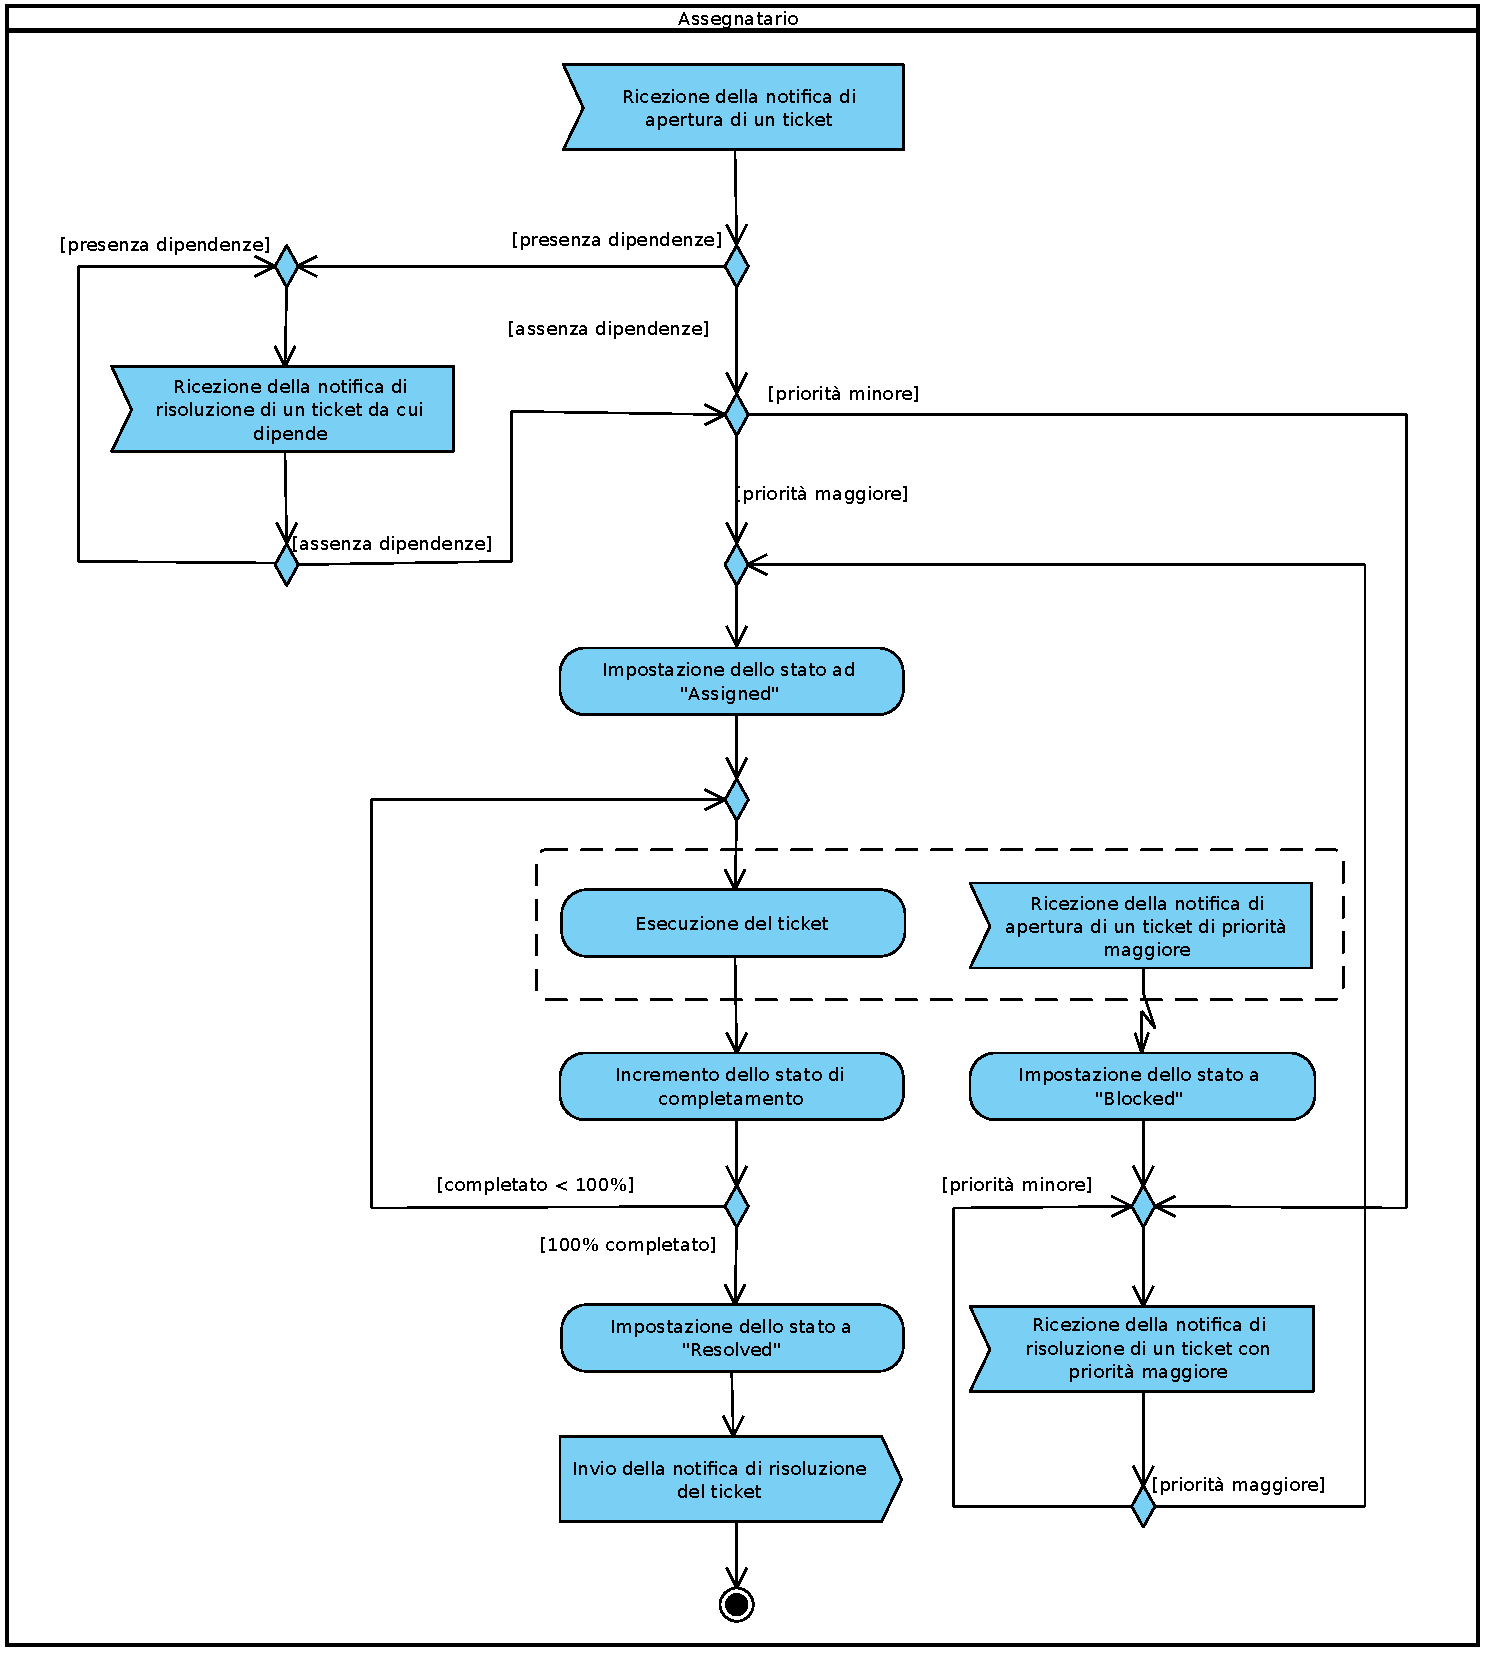
\includegraphics[width=13cm]{../immagini/lavorazioneTicket.pdf}
\caption{Diagramma di attività - lavorazione di un ticket}
\label{fig:lavorazioneTicket}
\end{figure}
\subsubsubsection{Protocollo di utilizzo dei ticket}\label{protocolloUtilizzo}
La procedura di lavorazione di un ticket da parte dell’assegnatario segue il diagramma
di attività riportato in \customRef{fig:lavorazioneTicket}{figura}.
\begin{enumerate}
\item Ogni membro, ricevuto almeno un ticket attivo, ne sceglierà uno prediligendo quelli a priorità maggiore e con scadenza più imminente;
\item Ogni utente non potrà avere più ticket in lavorazione contemporaneamente;
\item Nel caso in cui un utente ricevesse un ticket a scadenza più imminente rispetto a quello attualmente in lavorazione, dovrà sospendere il ticket corrente e iniziare a lavorare al ticket prioritario;
\item Una volta completato un ticket e dopo la sua verifica, se il \rV non ha individuato alcuna anomalia, allora potrà impostare lo stato del ticket ad ``Approved''. In caso contrario, seguirà la prassi descritta nella \customRef{procGestioneAnomalie}{sezione}, che è dedicata alle anomalie.
\end{enumerate}
\subsubsubsection{Ruoli di progetto}\label{ruoliProgetto}
I ruoli ricoperti dai vari componenti del gruppo varieranno ad ogni fase in modo tale che, alla fine del \gloxy{progetto}, ogni componente abbia rivestito ogni ruolo almeno una volta.
Tali ruoli sono stati stabiliti dal \rRP e saranno turnati secondo quanto previsto dalla seguente tabella.
\begin{table}
\tiny
\centering
\begin{tabular}{|>{\centering}>{\columncolor{gray!30}}m{1.4cm}|>{\centering}m{1.3cm}|>{\centering}m{1.3cm}|>{\centering}m{1.3cm}|>{\centering}m{1.3cm}|>{\centering}m{1.3cm}|>{\centering}m{1.3cm}|m{1.3cm}<{\centering}|}\hline
\textbf{Fasi} & \textbf{\gma} & \textbf{\ao} & \textbf{\mb} & \textbf{\dm} & \textbf{\gmi} & \textbf{\sm} & \textbf{\fv}\\\hline
\textbf{\fAt} & \makecell{\rRPt \\ \rAPt \\ \rVt} & \makecell{\rAPt \\ \rAt} & \makecell{\rAPt \\ \rAt} &  \makecell{\rRPt \\ \rAPt \\ \rAt \\ \rVt} & \makecell{\rAt \\ \rVt} & \makecell{\rAt \\ \rVt} & \makecell{\rRPt \\ \rAt \\ \rVt}\\\hline
\textbf{\fADt} & \makecell{\rAt \\ \rVt} & \rRPt & \rVt & \rAt & \makecell{\rAPt \\ \rVt} & \makecell{\rAt \\ \rVt} & \makecell{\rAt \\ \rVt}\\\hline
\textbf{\fPAt} & \makecell{\rPt \\ \rVt} & \makecell{\rPt \\ \rVt} & \rPt & \makecell{\rPt \\ \rVt} & \makecell{\rPt \\ \rVt} & \makecell{\rRPt \\ \rAPt \\ \rPt \\ \rVt} & \makecell{\rAt \\ \rVt}\\\hline
\textbf{\fPDt} & \makecell{\rAPt \\ \rAt \\ \rVt} & \makecell{\rPt \\ \rVt} & \makecell{\rRPt \\ \rPt \\ \rVt} & \makecell{\rPt \\ \rVt} & \rPt & \makecell{\rPt \\ \rVt} & \rPt\\\hline
\textbf{\fCt} & \makecell{\rPt \\ \rpt \\ \rVt} & \makecell{\rpt \\ \rVt} & \makecell{\rAt \\ \rPt \\ \rpt} & \makecell{\rpt \\ \rVt} & \makecell{\rRPt \\ \rAt \\ \rVt} & \makecell{\rPt \\ \rpt \\ \rVt} & \makecell{\rPt \\ \rVt}\\\hline
\textbf{\fVVt} & \makecell{\rPt \\ \rVt} & \makecell{\rAt \\ \rVt} & \makecell{\rPt \\ \rVt} & \makecell{\rRPt \\ \rVt} & \makecell{\rpt \\ \rVt} & \makecell{\rAPt \\ \rVt} & \makecell{\rpt \\ \rVt}\\\hline
\end{tabular}
\caption{Rotazione ruoli di progetto.}
\label{tabella:rotazioneRuoli}
\end{table}
Deve valere sempre la seguente condizione: \emph{un componente che abbia preso come incarico la stesura di uno specifico documento o la scrittura di uno particolare file di codice sorgente non potrà, in alcun modo, risultare come \rV dello stesso}. \\
Questa norma garantisce l'assenza di conflitto di interessi nello svolgimento delle successive attività di verifica e di approvazione all'interno del gruppo.\\
\subsubsubsubsection{\rRP}
Il \rRP ha il compito di mantenere i contatti con gli enti esterni al gruppo, e detiene il potere decisionale, quindi ha responsabilità su:
\begin{itemize}
\item Pianificazione, coordinamento e controllo delle attività;
\item Gestione delle risorse;
\item Analisi e gestione dei rischi;
\item Approvazione dei documenti;
\item Approvazione dell'offerta economica;
\item Redazione del \PP e collabora alla stesura del \PQ, in particolare nella sezione relativa alla pianificazione.
\end{itemize}
Si assicura che le attività di verifica vengano svolte sistematicamente seguendo le \NP, vengano rispettati i ruoli e le competenze assegnate nel \PP, non vi siano conflitti di interesse tra redattori e \rVs. \`E l'unico a poter decidere l'approvazione di un documento e a sancirne la distribuzione.
Ha inoltre l'incarico di gestire la creazione e l'assegnazione dei ticket delle macro-fasi e di assegnare ad un membro del gruppo il ruolo di responsabile di quest'ultima.
\subsubsubsubsection{\rAP}
L'\rAP è il responsabile dell'ambiente di lavoro e le sue principali mansioni sono:
\begin{itemize}
\item Ricerca di strumenti che possano automatizzare qualsiasi compito automatizzabile;
\item Risoluzione dei problemi legati alle difficoltà di gestione e controllo dei processi e delle risorse, poiché la loro risoluzione richiede l'adozione di strumenti software adatti;
\item Controllo delle versioni e delle configurazioni del prodotto;
\item Gestione dell'archiviazione e del \gloxy{versionamento} della documentazione di \gloxy{progetto}, attraverso l'uso di database;
\item Scelta di procedure e strumenti per il monitoraggio e la segnalazione per il controllo qualità;
\item Redazione delle \NP, dove spiega e norma l'utilizzo degli strumenti, redige la sezione del \PQ dove vengono descritti strumenti e metodi di verifica.
\end{itemize}
\subsubsubsubsection{\rA}
L’\rA è il responsabile delle attività di analisi e le sue responsabilità principali sono:
\begin{itemize}
\item Produzione di una specifica di \gloxy{progetto} comprensibile e motivata in ogni suo punto;
\item Comprensione esaustiva della natura e della complessità del problema;
\item Redazione dello \SF, dell'\AR e parte del \PQ. Partecipa alla redazione del \PQ in quanto conosce l'ambito del \gloxy{progetto} ed ha chiari i livelli di qualità richiesta e le procedure da applicare per ottenerla.
\end{itemize}
\subsubsubsubsection{\rP}
Il \rP è il responsabile delle attività di progettazione e le sue responsabilità sono:
\begin{itemize}
\item Produzione di una soluzione attuabile che sia comprensibile, robusta e semplice;
\item Scelta dei \gloxy{design pattern} da impiegare;
\item Scelta degli aspetti progettuali e tecnologici che rendano il prodotto facilmente manutenibile;
\item Scelta degli aspetti progettuali e tecnologici che rendano il prodotto modulare entro i limiti del possibile;
\item Redazione della \ST, della \DP e delle sezioni inerenti le metriche di verifica della programmazione del \PQ.
\end{itemize}
\subsubsubsubsection{\rp}
Il \rp è il responsabile delle attività di codifica e delle componenti di ausilio necessarie per l'esecuzione delle prove di verifica e validazione. Le sue responsabilità sono:
\begin{itemize}
\item Implementazione rigorosa delle soluzioni descritte dal \rP, da cui seguirà la realizzazione del prodotto;
\item Scrittura di codice documentato, versionato, manutenibile e che rispetti gli standard stabiliti per la scrittura del codice;
\item Implementazione dei test sul codice scritto, necessari per le prove di verifica e validazione;
\item Redazione del \MU.
\end{itemize}
\subsubsubsubsection{\rV}
Il \rV il è responsabile delle attività di verifica. Effettua la verifica dei documenti utilizzando gli strumenti e i metodi proposti dal \PQ e attenendosi a quanto descritto nelle \NP. Le responsabilità di tale ruolo sono:
\begin{itemize}
\item Controllo di conformità dell'attuazione delle attività con le norme stabilite;
\item Controllo di conformità di ogni stadio del ciclo di vita del prodotto;
\item Redazione della sezione del \PQ, che illustra l'esito e la completezza delle verifiche e delle prove effettuate.
\end{itemize}
